\documentclass[a4paper,12pt]{article}

% Packages
\usepackage[french]{babel}   % Langue française
\usepackage[T1]{fontenc}     % Encodage des caractères
\usepackage{lmodern}         % Police plus agréable
\usepackage{amsmath}         % Mathématiques
\usepackage{graphicx}        % Images
\usepackage{hyperref}        % Liens hypertextes
\usepackage{geometry}        % Gestion des marges
\geometry{margin=2.5cm}      % Marges ajustées
\usepackage{fancyhdr}        % En-têtes/pieds de page
\usepackage{xcolor} 
\usepackage{hyperref}        

% Configuration des en-têtes et pieds de page
\pagestyle{fancy}
\fancyhead[L]{Projet Calcul Parallèle 2024/2025}
\fancyhead[R]{}
\fancyfoot[C]{\thepage}

% Début du document
\begin{document}

% Titre
\begin{center}
    {\LARGE \textbf{Projet Calcul Parallèle 2024/2025}} \\
    \vspace{0.5cm}
    {\Large \textbf{Rapport de Projet}} \\
    \vspace{1cm}
    \textbf{Auteur : [Mohamad SAMMAN]} \\
    \textbf{Encadrant : [S.ABIDE]} \\
    \vspace{1cm}
    \textbf{\today}
\end{center}

\section{Introduction}
Ce projet vise à explorer le calcul parallèle à travers l’installation et l’utilisation des bibliothèques \textbf{HDF5} et \textbf{Decomp2d}. Après une première validation d’un code séquentiel utilisant la méthode des différences finies et le gradient conjugué, nous avons parallélisé les calculs avec \textbf{Decomp2d}. 

\section{Mise en place de l’environnement}
L’installation des bibliothèques s’est faite en deux étapes :
\begin{itemize}
    \item \textbf{HDF5} : Permet d’écrire des données en parallèle.
    \item \textbf{Decomp2d} : Utilisée pour distribuer des tableaux 3D sur une grille de processeurs 2D.
\end{itemize}


\section{Validation du code séquentiel}
Avant d’aborder le calcul parallèle, nous avons validé notre méthode sur un cas test basé sur une \textbf{solution fabriquée} (Méthode de la Solution Manufacturée - MMS) :
\begin{itemize}
    \item Utilisation des \textbf{différences finies centrées} pour approximer les dérivées secondes. (ordre 2 grace à la symétrisation)
    \item Résolution du système par la \textbf{méthode du gradient conjugué}.
\end{itemize}
Les résultats sont illustrés par les graphes de la Figure (\ref{fig:validation}). La solution FD est plus lisse.\\
La différence de l'échelle pour les deux graph provient du fait que nous avons utilisé le nombre de point (nx et ny) pour la méthode CG et les coordonées (x et y) pour FD. Le domaine étant identique pour les deux méthodes: [0,1]x[0,1]

\begin{figure}[h]
    \centering
    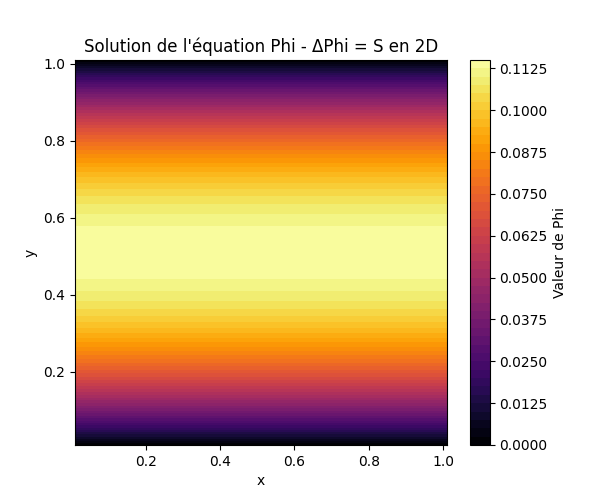
\includegraphics[width=0.45\textwidth]{1.png}
    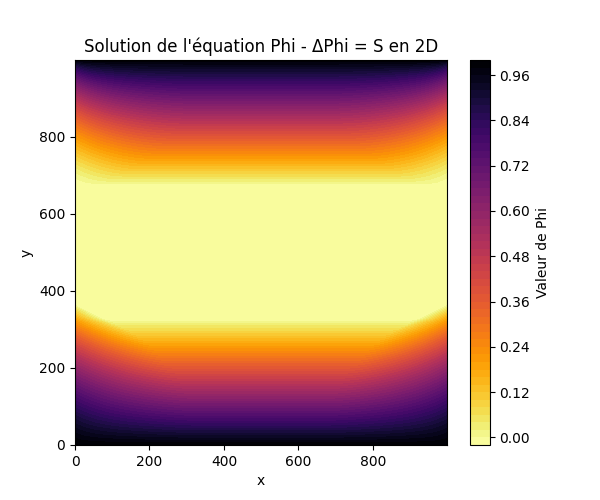
\includegraphics[width=0.45\textwidth]{2.png}
    \caption{Résultats obtenus avec les différences finies (gauche) et le gradient conjugué (droite).}
    \label{fig:validation}
\end{figure}

\newpage
\section{Concepts de Strong Scaling et Weak Scaling}
Nous expliquons ces notions théoriquement et ensuite regardons les courbes de scalling.

\subsection{Strong Scaling}
Le \textbf{strong scaling} mesure l’accélération obtenue en augmentant le nombre de cœurs tout en conservant une taille de problème fixe :
\begin{equation}
S_s = \frac{T_1}{T_p}
\end{equation}
où $T_1$ est le temps d’exécution en séquentiel et $T_p$ en parallèle.

\paragraph{Allure attendue de la courbe :}  
\begin{itemize}
    \item \textbf{Parallélisation idéale :} L’accélération est linéaire : en doublant le nombre de cœurs, le temps d’exécution est divisé par 2.
    \item \textbf{Parallélisation sous-optimale :} La courbe commence par suivre la tendance linéaire mais atteint une saturation due aux \textbf{communications entre processeurs} et aux \textbf{surcharges parallèles}.
    \item \textbf{Mauvaise parallélisation :} Peu ou pas d’amélioration, voire un ralentissement si la surcharge de communication dépasse le gain du calcul parallèle.
\end{itemize}
Nous pouvons observer une allure typique du strong scalling Figure (\ref{strong}) provenant de \cite{scaling-site}


\subsection{Weak Scaling}
Le \textbf{weak scaling} analyse l’évolution du temps d’exécution lorsqu’on augmente la taille du problème proportionnellement au nombre de cœurs :
\begin{equation}
S_w = \frac{T_p(N)}{T_p(N/P)}
\end{equation}
où $N$ est la taille du problème et $P$ le nombre de cœurs.

\paragraph{Allure attendue de la courbe :}  
\begin{itemize}
    \item \textbf{Parallélisation efficace :} Le temps d’exécution reste constant, car la charge de travail par processeur reste la même.
    \item \textbf{Parallélisation inefficace :} Le temps d’exécution augmente progressivement à cause des \textbf{latences de communication} et de la \textbf{gestion de la mémoire partagée}.
\end{itemize}
Nous pouvons observer une allure typique du weak scalling Figure (\ref{weak}) provenant de \cite{scaling-site}

\section{Conclusion et perspectives}
Nous avons réussi à valider l’algorithme séquentiel et à coder la paraléllisation avec la librarie \textbf{Decomp2d}. Pour la suite, il serait pertinent de :
\begin{itemize}
    \item Étudier les communications entre processus pour optimiser le code parallèle.
    \item Implémenter le code pour d'autres types de problèmes.
\end{itemize}

\begin{figure}[h]
    \centering
    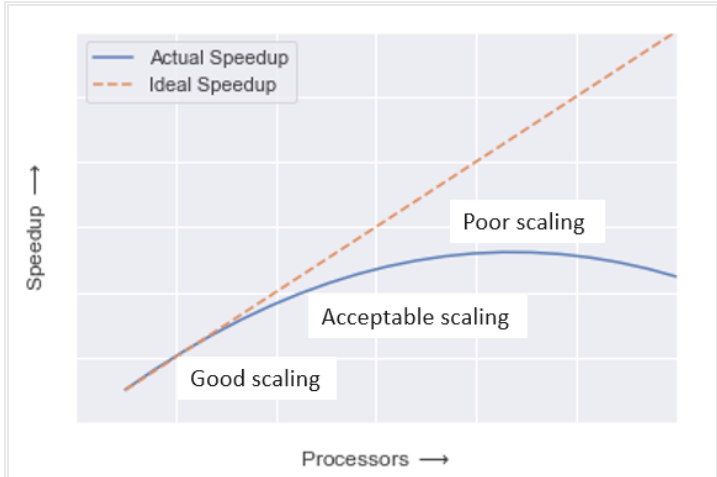
\includegraphics[width=0.6\textwidth]{3.png}
    \caption{Allure typique d’une courbe de strong scaling.}
    \label{strong}
\end{figure}

\begin{figure}[h]
    \centering
    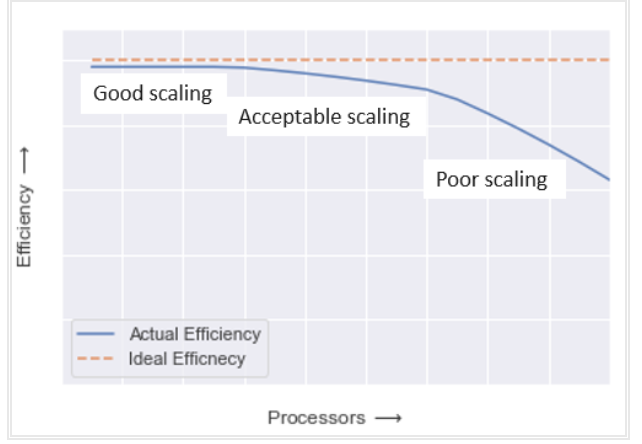
\includegraphics[width=0.6\textwidth]{4.png}
    \caption{Allure typique d’une courbe de weak scaling.}
    \label{weak}
\end{figure}
\\
\newpage
\begin{thebibliography}{9}
    \bibitem{scaling-site} Scaling experiments: How to measure the performance of parallel code on HPC systems. Water Programming. \href{https://waterprogramming.wordpress.com/2021/06/07/scaling-experiments-how-to-measure-the-performance-of-parallel-code-on-hpc-systems/}{https://waterprogramming.wordpress.com/2021/06/07/scaling-experiments-how-to-measure-the-performance-of-parallel-code-on-hpc-systems/}
\end{thebibliography}

\end{document}
